\documentclass[12pt]{ximera}

\usepackage{nopageno}
\usepackage{amsmath}
\usepackage{graphicx}
\usepackage{geometry}
\geometry{top=1in,bottom=1in,right=0.75in,left=0.75in}
\usetikzlibrary{patterns}

\usepackage{fancyhdr}
\usepackage{lastpage}
 
\pagestyle{fancy}
\fancyhf{}
\rhead{\textsf{Form D}}
\lhead{\textsf{Calculus Knowledge Assessment v3}}
\rfoot{\textsf{Page \thepage\ of \pageref{LastPage}}}


\usepackage{multicol}
\setlength{\columnsep}{2cm}

\usepackage{enumitem}

\setitemize{noitemsep,topsep=0pt,parsep=0pt,partopsep=0pt}

\renewenvironment{multipleChoice}
{\begin{trivlist}\item[\hskip\labelsep\small\bfseries Choose the best answer:]
\hfil\begin{enumerate}\begin{multicols}{2}}
 {\end{multicols}\end{enumerate}\end{trivlist}}

\def\image{\begin{center}}
\def\endimage{\end{center}}

%\renewcommand{\choice}[2][]{\item \begin{minipage}[t]{2in}#2\end{minipage}\ifthenelse{\boolean{#1}}{\ifhandout \else \quad\checkmark\fi}{}}
\renewcommand{\choice}[2][]{\item \begin{minipage}[t]{2in}#2\end{minipage}\ifthenelse{\boolean{#1}}{\ifhandout \else  \fi}{}}


\begin{document}
\vspace{6ex}

\begin{minipage}{\textwidth}
\begin{problem}
  %\GoodQuestions{Subject: Continuity and the Intermediate Value Theorem 4Q}
  You know the following statement is true: ``If $f$ is a
    polynomial function, then $f$ is a continuous function.''  Which
    of the following must also be true?
  \begin{multipleChoice}
     \choice[correct]{If $f$ is not continuous, then it is not a polynomial.}
     \choice{If $f$ is continuous, then it is a polynomial.}
     \choice{If $f$ is not a polynomial, then it is not continuous.}
     \choice{None of the above.}
  \end{multipleChoice}
\end{problem}
\end{minipage}

\vspace{6ex}

\begin{minipage}{\textwidth}
\begin{problem}
  %\GoodQuestions{Subject: Tangents, velocities, and other rates of change 2P}
  What can be said about the line tangent to the graph of $f(x)=x$ at $(0,0)$?
  \begin{multipleChoice}
  \choice{It is $y=0$.}
  \choice{It is $y=1$.}
  \choice[correct]{It is $y=x$.}
  \choice{It does not exist.}
  \choice{It is not unique. There are infinitely many tangent lines.}
  \end{multipleChoice}
\end{problem}
\end{minipage}

\vspace{6ex}

\begin{minipage}{\textwidth}
\begin{problem}
  The graph below is a plot of a function $f$.  What best describes
  the behavior of $f$ on the interval from $x=-2$ to $x=2$?
  \begin{image}
    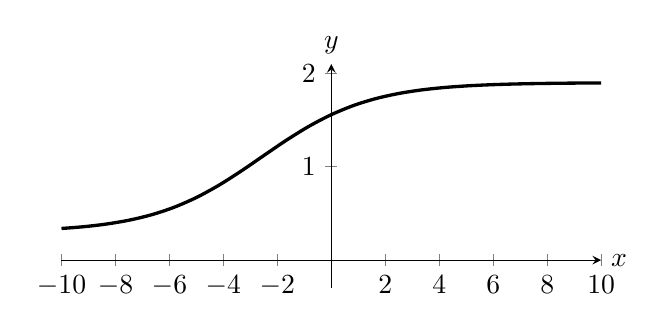
\begin{tikzpicture}
      \begin{axis}[
        clip=false,
        y post scale=0.5,
        domain=-10:10, 
        ytickmin=0,ytickmax=3,
        ytick={1,2},
        xtickmin=-10,xtickmax=10,
        xtick={-10,-8,-6,-4,-2,2,4,6,8,10},
        ymin=-0.3, ymax=2.1,
        xlabel=$x$, ylabel=$y$,
        axis lines=center,
        every axis y label/.style={at=(current axis.above origin),anchor=south},
        every axis x label/.style={at=(current axis.right of origin),anchor=west},
        axis on top,
        ]          
        \addplot [very thick,smooth] {0.3 + 1.6/(1 + exp(-0.5*(x + 2.6))};
      \end{axis}
    \end{tikzpicture}
    \end{image}
  \begin{multipleChoice}
    \choice{As $x$ increases, $f(x)$ is increasing at an increasing rate.}
    \choice[correct]{As $x$ increases, $f(x)$ is increasing at a decreasing rate.}
    \choice{As $x$ increases, $f(x)$ is increasing at a constant rate.}
    \choice{As $x$ increases, $f(x)$ is decreasing at a decreasing rate.}
    \choice{As $x$ increases, $f(x)$ is decreasing at an increasing rate.}
  \end{multipleChoice}
\end{problem}
\end{minipage}

\vspace{6ex}

\begin{minipage}{\textwidth}
\begin{problem}

  Four numbers are shown below.
  \begin{image}
    \begin{tikzpicture}[x=0.19\textwidth]
      \draw[-{>[scale=1.75]}] (-0.05\textwidth,0) -- (0.8\textwidth,0);
      \foreach \x in {0,...,4} {%
        \draw (\x,-.1) -- (\x,.1);
        \node[anchor=north,yshift=-2pt] at (\x,0) {$\x$};
      }
      \draw (3.141592654,-.1) -- (3.141592654,.1);
      \node[anchor=north,yshift=-2pt] at (3.141592654,0) {$\pi$};
      \draw (0.25,0) node [circle,fill,inner sep=1pt,label=above:$x$](e){};
      \draw (0.65,0) node [circle,fill,inner sep=1pt,label=above:$y$](e){};
      \draw (3.3,0) node [circle,fill,inner sep=1pt,label=above:$z$](e){};
      \draw (3.8,0) node [circle,fill,inner sep=1pt,label=above:$w$](e){};
    \end{tikzpicture}
  \end{image}
  Let $f(x) = \sin x$.  What is true about $f(x)$, $f(y)$, $f(z)$, and $f(w)$?
  \begin{multipleChoice}
    \choice{$f(x) > f(y) > f(z) > f(w)$.}
    \choice{$f(x) > f(y) > f(w) > f(z)$.}
    \choice[correct]{$f(y) > f(x) > f(z) > f(w)$.}
    \choice{$f(y) > f(x) > f(w) > f(z)$.}
  \end{multipleChoice}
\end{problem}
\end{minipage}

\vspace{6ex}

\begin{minipage}{\textwidth}
\begin{problem}

  Suppose whenever $x$ is very large, $f(x)$ is close to 1.  What is true about $f$?
  \begin{multipleChoice}
    \choice{The graph of $f$ does not cross the line $y = 1$.}
    \choice{The graph of $f$ does not cross the line $x = 1$.}
    \choice{Whenever $x$ is close to zero, $f(1/x)$ is close to 1.}
    \choice[correct]{Whenever $x$ is very large, $f(x^2)$ is close to 1.}
  \end{multipleChoice}
\end{problem}
\end{minipage}

\vspace{6ex}

\begin{minipage}{\textwidth}
\begin{problem}

  Shown below is the graph of $y = e^x$ and a tangent line $y = mx + b$ to the graph passing through the point $(8,e^8)$.
  \begin{image}
    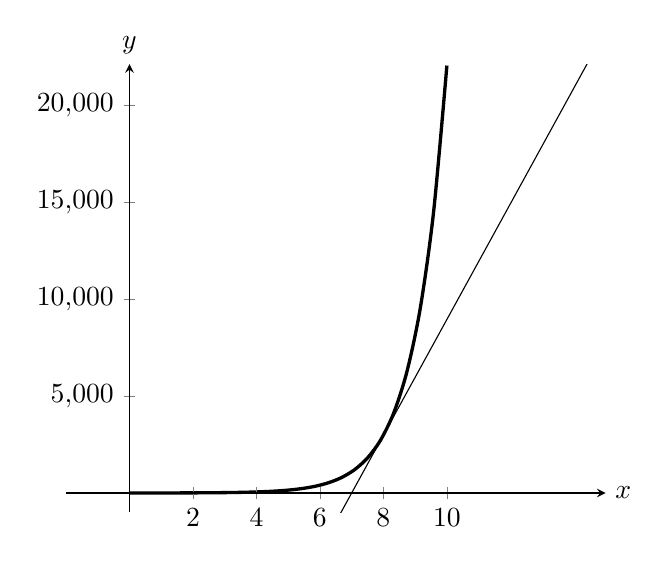
\begin{tikzpicture}
      \begin{axis}[
        clip=true,
        domain=0:10,
        ytickmin=0,ytickmax=20000,
        xtickmin=0,xtickmax=10,
        ymin=-1000, ymax=22100,
        xmin=-2, xmax=15,
        ytick={5000,10000,15000,20000},
        scaled y ticks=false,
        xlabel=$x$, ylabel=$y$,
        axis lines=center,
        every axis y label/.style={at=(current axis.above origin),anchor=south},
        every axis x label/.style={at=(current axis.right of origin),anchor=west},
        axis on top,
        ]          
        \addplot [very thick,smooth] {exp(x)};
        \addplot [smooth,domain=0:15] {exp(8)*(x-8) + exp(8)};
      \end{axis}
    \end{tikzpicture}  
  \end{image}
  How does $200m + b$ compare to $e^{200}$?
  \begin{multipleChoice}
    \choice{$200m + b$ equals $e^{200}$.}
    \choice{$200m + b$ is bigger than $e^{200}$.}
    \choice{$200m + b$ is a little bit smaller than $e^{200}$.}
    \choice[correct]{$200m + b$ is much smaller than $e^{200}$.}
  \end{multipleChoice}
\end{problem}
\end{minipage}

\vspace{6ex}

\begin{minipage}{\textwidth}
\begin{problem}
  Suppose the slope of a tangent line to the graph of $f$ at the point $x$ is $x \cdot f(x)$ and suppose $f(0) = 1$.  What must be true of $f$?
  \begin{multipleChoice}
    \choice[correct]{By choosing $x$ large enough, $f(x)$ can be made as large as desired}
    \choice{By choosing $x$ large enough, $f(x)$ can be made as close to zero as desired}
    \choice{By choosing $x$ large enough, $f(x)$ can be made as negative as desired}
  \end{multipleChoice}
\end{problem}
\end{minipage}

\vspace{6ex}

\begin{minipage}{\textwidth}
\begin{problem}
  Suppose $f$ and $g$ are two functions with the same derivative at every point.  What quantity below is the best guess for the value of $g(0.998)$?
  \begin{multipleChoice}
    \choice{$g(1) + f(1.02) - f(1)$}
    \choice{$g(1) + f(1) - f(1.02)$}
    \choice[correct]{$g(1) + 2\, f(1) - 2\, f(1.001)$}
    \choice{$g(1) + 2\, f(1.001) - 2\, f(1)$}
  \end{multipleChoice}
\end{problem}
\end{minipage}

\vspace{6ex}

\begin{minipage}{\textwidth}
\begin{problem}
  Suppose $f$ is a function (with domain consisting of nonzero real numbers) so that $f'(x) = 1/x$.  What must be true of $f$?
  \begin{multipleChoice}
    \choice{$f(x) = \ln x$}
    \choice{$f(x) = \ln |x|$}
    \choice{There is a number $C$ (possibly zero) so that $f(x) = C + \ln x$}
    \choice{There is a number $C$ (possibly zero) so that $f(x) = C + \ln |x|$}
    \choice[correct]{$\frac{d}{dx} \left( f(x) - \ln |x| \right) = 0$}
  \end{multipleChoice}
\end{problem}
\end{minipage}

\vspace{6ex}

\begin{minipage}{\textwidth}
\begin{problem}
  Suppose $f(a)$ is the area of the region bounded by $x^2 + y^2 \leq 25$ and $-5 \leq x \leq a$.  What integer is closest to $\frac{f(4.01) - f(4)}{0.01}$?
  \begin{multipleChoice}
    \choice{3}
    \choice{4}
    \choice{5}
    \choice[correct]{6}
  \end{multipleChoice}
\end{problem}
\end{minipage}

\vspace{6ex}

\begin{minipage}{\textwidth}
\begin{problem}
  Suppose $f$ is a continuous function.  Consider $g(n) = \int_0^1 f(x^n) \, dx$.  When $n$ is very large, what is a good guess as to the value of $g(n)$?
  \begin{multipleChoice}
    \choice[correct]{When $n$ is large, $g(n)$ is close to $f(0)$}
    \choice{When $n$ is large, $g(n)$ is close to $f(1)$}
    \choice{When $n$ is large, $g(n)$ is close to the average value of $f$ on the interval $[0,1]$}
  \end{multipleChoice}
\end{problem}
\end{minipage}

\vspace{6ex}

\begin{minipage}{\textwidth}
\begin{problem}
  Suppose $z = 10^{10}$ and $x = \sqrt{z}$ and $y = \sqrt{x}$.  What number below is closest to $x/y$?
  \begin{multipleChoice}
    \choice{$10$}
    \choice{$30$}
    \choice{$100$}
    \choice[correct]{$300$}
  \end{multipleChoice}
\end{problem}
\end{minipage}

\vspace{6ex}

\begin{minipage}{\textwidth}
\begin{problem}
  Suppose $x = \frac{5 + \sqrt{0.1}}{200}$ and $y = \frac{21}{10}$.  What integer is closest to $x - y$?
  \begin{multipleChoice}
    \choice{$-26$}
    \choice{$-21$}
    \choice{$-16$}
    \choice[correct]{$-2$}
    \choice{$200$}
  \end{multipleChoice}
\end{problem}
\end{minipage}

\vspace{6ex}

\begin{minipage}{\textwidth}
\begin{problem}
	Let $f$ and $g$ be two functions satisfying the relationship $f(5x) = g(x)$.  Suppose the point $(1,2)$ is on the graph of $f$.
	\begin{multipleChoice}
		\choice{The point $(5, 2)$ is on the graph of $g$}
		\choice{The point $(5, 10)$ is on the graph of $g$}
		\choice{The point $(\frac{1}{5}, 10)$ is on the graph of $g$}
		\choice[correct]{The point $(\frac{1}{5},2)$ is on the graph of $g$}
	\end{multipleChoice}
\end{problem}
\end{minipage}

\vspace{6ex}

\begin{minipage}{\textwidth}
\begin{problem}
	Let $f$ be the function defined by $f(x) = x^2+1$, and $g$ be the function defined by the rule $g(z) = z^2+1$. 
	\begin{multipleChoice}
		\choice{Since $f$ and $g$ have differing domain, they are different functions}
		\choice[correct]{$f$ and $g$ are the same function}
		\choice{$f$ and $g$ are different functions because they disagree for some inputs in their common domain}
		\choice{$f$ and $g$ are different functions because they are of different variables}
	\end{multipleChoice}
\end{problem}
\end{minipage}

\vspace{6ex}

\begin{minipage}{\textwidth}
\begin{problem}
	Suppose $x$ is a small negative number.  What can be said about $\frac{x}{|x|}$?
	\begin{multipleChoice}
		\choice[correct]{It is close to $-1$}
		\choice{It is close to $1$}
		\choice{It is close to $0$}
	\end{multipleChoice}
\end{problem}
\end{minipage}

\vspace{6ex}

\begin{minipage}{\textwidth}
\begin{problem}
  Suppose $x$ is a number close to zero, and $y$ is a very large number.  What can be said about $y/x$?
  \begin{multipleChoice}
    \choice{It is very large.}
    \choice{It is close to zero.}
    \choice{It is very negative.}
    \choice[correct]{It could be very positive or very negative.}
  \end{multipleChoice}
\end{problem}
\end{minipage}

\vspace{6ex}

\begin{minipage}{\textwidth}
\begin{problem}
  Suppose $A$ and $a$ differ by at most $2$ and suppose $B$ and $b$
  differ by at most $1$.  In symbols, this means that $|A - a| < 2$ and $|B - b| < 1$.
  By how much could $A/B$ and $a/b$ differ?
  \begin{multipleChoice}
    \choice{By no more than $1$, meaning $|A/B - a/b| < 1$}
    \choice{By no more than $2$, meaning $|A/B - a/b| < 2$}
    \choice{By no more than a factor of $2$, meaning $\left| \frac{A/B}{a/b} \right| < 2$}
    \choice{By no more than a factor of $1/2$, meaning $\left| \frac{A/B}{a/b} \right| < \frac{1}{2}$}
    \choice[correct]{By any amount}
  \end{multipleChoice}
\end{problem}
\end{minipage}

\vspace{6ex}

\begin{minipage}{\textwidth}
\begin{problem}
  Suppose $f$ and $g$ are continuous functions.  Let $h(x) = \frac{f(x+0.01) \cdot g(x - 0.01)}{f(x-0.02) \cdot f(x + 0.02)}$.  Without knowing anything else, what number below is the best guess for $h(2)$?
  \begin{multipleChoice}
    \choice{$f(2)$}
    \choice{$g(2)$}
    \choice{$f(2)/g(2)$}
    \choice[correct]{$g(2)/f(2)$}
  \end{multipleChoice}
\end{problem}
\end{minipage}

\vspace{6ex}

\begin{minipage}{\textwidth}
\begin{problem}
  Suppose $p(x) = x^2 + a$ is a quadratic polynomial.  If $a > 0$, is it possible that there is a point $x$ so that $p'(x) = p(x) = 0$?
  \begin{multipleChoice}
    \choice{Yes}
    \choice[correct]{No}
  \end{multipleChoice}
\end{problem}
\end{minipage}

\end{document}

%%% Local Variables:
%%% mode: latex
%%% TeX-master: t
%%% End:
